\chapter{Monte Carlo Methods}
\graphicspath{{Chapter2/figures/}}
\label{ch:mcmethods}
Monte Carlo Methods have achieved significant success in its application to various domains in the last few decades. This chapter reviews some fundamental concept in Monte Carlo method that are related to this thesis. It first begins with a summary on the main concept of Bayesian inference. It then discusses some  basic Monte Carlo methods such as perfect Monte Carlo sampling, rejection sampling, importance sampling. Lastly, it details the Sequential Monte Carlo (SMC), along with various enhancement made to the techniques, used in this thesis.

\section{Bayesian Inference}
In Bayesian inference, each unknown parameter in the model is assumed to be random variable and is associated with a prior distribution that characterises the initial belief. The inference process is merely about updating the belief with new observable evidence in a systematic fashion using Bayes theorem.

Formally, let $\mathcal{M}$ be the model used, $\theta$ be the set of parameters of the model, $p\left(\theta \mid \mathcal{M}\right)$ be the prior distribution (initial belief) and $p(x \mid \theta, \mathcal{M})$ be the likelihood (probability of observing an observation $x$ given the model) then posterior distribution (updated belief) is given as follows:  
\begin{align}
  p(\theta \mid x , \mathcal{M}) &= \frac{p(x \mid \theta , \mathcal{M})~p(\theta \mid \mathcal{M})}{p(x \mid \mathcal{M})} \nonumber \\
                   &\propto p(x \mid \theta , \mathcal{M})~p(\theta \mid \mathcal{M}) \label{eq:bayes} \\
  \text{posterior} &\propto \text{likelihood} \times \text{prior}
\end{align}

This problem formulation is elegant, but there remains some subtle issues in practice. One particular issue is the calculation of the normalisation constant $p(x \mid \mathcal{M})$ in \eqref{eq:bayes}, which demands us to be able to carry out the following integral  analytically:
\begin{equation}
  p(x \mid \mathcal{M}) = \int p(x \mid \theta, \mathcal{M}) p(\theta \mid \mathcal{M})~d\theta
\end{equation}
This is often infeasible. A often way to circumvent this requirement is by making use of conjugate prior that yields posterior distributions from the same family in an analytical fashion. Moreover, the need of calculating integral that does not possess analytic solution also arises in the marginalisation process of nuisance parameters, calculating expectation of a function, etc.

\section{Perfect Monte Carlo}
Instead of a closed form solution, the Method Carlo methods offer a numerical solution in estimating the integral using simple sampling techniques. Consider the calculation the expectation of a function, $I$ of the following form:
\begin{equation}
  I = \E_p[f(x)] = \int f(x)p(x)~dx
\label{eq:expectation}
\end{equation}
Assuming we are able to sample $N$ independent and identically distributed (i.i.d.) samples of $x$ from $p(\cdot)$, denote these as $\{x^{(i)}\}$ where $i \in \{1 \ldots N\}$, a Monte Carlo estimate of $I$ using the the point masses of the samples is:
\begin{equation}
  \hat{I} = \frac{1}{N} \sum^N_{i=1} f(x^{(i)})
\end{equation}
This approximation can be viewed as discretization of the continuous distribution with \emph{random} grid points. This estimate is unbiased and converge almost surely to $I$ as $N \to \infty$ by the Law of Large number \cite{RCP05}. 

Moreover, if the variance of $f(\cdot)$ is bounded ($\sigma^2_f < \infty$), as $N \to \infty$, then the following central limit theorem holds:
\begin{equation}
  \sqrt{N}(\hat{I} - I) \Longrightarrow N(0, \sigma^2_f)
\end{equation}
where $\Longrightarrow$ denotes convergence in distribution \cite{AD09}. The key point to note here is this convergence rate of $\frac{1}{\sqrt{N}}$ is independent of the dimensions of $x$. This is in contrast with any deterministic method that has a rate that decreases as the integral dimension increases \cite{RCP05}. This is the main advantage of Monte Carlo integration.

\section{Rejection sampling}
However, it is not always possible to sample directly from the distribution $p(\cdot)$. Suppose we can find an instrumental distribution (a.k.a. proposal distribution), $q(\cdot)$, that is easy to sample from and has the property such that $cq(x)$ dominates $p(x)$ for all $x$, i.e., $cq(x) \geq p(x) \geq 0$ for all $x$, then to get a random sample from $p(\cdot)$, we can first sample from $q(\cdot)$ instead and accept the sample with acceptance probability $\alpha(x)=\dfrac{p(x)}{cq(x)}$. If the sample is rejected, the process is repeated until success. This rejection algorithm is summarised in Algorithm \ref{algo:rejectionsampling}\footnote{The set notation is used here, despite it is actually a collection that allows duplicates. Therefore, the $\cup$ operation should be viewed as a simple join of two collections.}.

\begin{algorithm}
\caption{Rejection Sampling}\label{algo:rejectionsampling}
\begin{algorithmic}[1]
\Function{RejectionSampling}{N}
\State $\mathcal{X} = \{\ \}$.
\Repeat
  \State sample $x \sim q(\cdot)$.
  \State sample $u \sim \mathcal{U}(0,1)$.
  \If {$u \leq \dfrac{p(x)}{cq(x)}$}.
    \State $\mathcal{X} \gets \mathcal{X} \cup \{x\}$.
  \EndIf
\Until{len($\mathcal{X}$)=N}.
\State return $\mathcal{X}$.
\EndFunction
\end{algorithmic}
\end{algorithm}

Looking at the acceptance ratio formula, it is not difficult to see that the optimal instrumental distribution, $q^*$, is the one that minimizes the space bounded by $cq(x)$ subject to the constraint that it still dominates the target density $p(x)$. As the dimension of $x$ increases, this algorithm becomes very inefficient because the acceptance ratio which is essentially defined as the ratio of two spaces tends towards zero. Therefore, many generated examples would be rejected. 

\section{Importance sampling}
\label{sec:IS}
Instead of making a binary accept-reject decision on each sample, the key concept in important sampling is assign weighting to each sample (obtained from the instrumental distribution, $q(\cdot)$) based on how well the sample resembles the target distribution, $p(\cdot)$. More formally, assume we have an instrumental distribution, $q(\cdot)$ that has support that includes $p(\cdot)$, we can re-write \eqref{eq:expectation} as:
\begin{align}
  I &= \int f(x)\dfrac{p(x)}{q(x)}q(x)~dx \nonumber \\
    &= \int f(x)w(x)q(x)~dx \nonumber \\
    &= \E_q[f(x)w(x)]
\end{align}
where $w(x)$ is commonly referred as the importance weight. This reformulation leads to the following Monte Carlo estimate of $I$:
\begin{align}
  \hat{I} &= \dfrac{\frac{1}{N} \sum^N_{i=1} \tilde{w}(x^{(i)})f(x^{(i)})}{\frac{1}{N} \sum^N_{j=1} \tilde{w}(x^{(j)})} \nonumber \\ 
          &= \sum^N_{i=1} \dfrac{\tilde{w}(x^{(i)})}{\sum^N_{j=1} \tilde{w}(x^{(j)})} f(x^{(i)}) \nonumber \\
          &= \sum^N_{i=1} \hat{w}(x^{(i)}) f(x^{(i)})  \label{eq:is} 
\end{align}
where $\tilde{w}(x^{(i)}) = \dfrac{p(x^{(i)})}{q(x^{(i)})}$ and $\hat{w}(x^{(i)})  = \dfrac{\tilde{w}(x^{(i)})}{\sum^N_{j=1} \tilde{w}(x^{(j)})}$ are referred to as unnormalized and normalised importance weight respectively \cite{CO05}. This estimate is biased as it consists of the ratio of two estimates, yet it is still asymptotically consistent.

To obtain samples from the target distribution, $p(\cdot)$, an additional resampling step can be introduced. In the first step, we draw a set of samples $\{\tilde{x}^{(i)}\}$ from the instrumental distribution and compute their associated normalised importance weights, $\hat{w}(\tilde{x}^{(i)})$. In the resampling step, we draw the final sample set, $\{x^{(i)}\}$ from this intermediate set of samples by taking into account the importance weights. This importance sampling algorithm is summarised in Algorithm \ref{algo:importancesampling}

\begin{algorithm}
\caption{Importance Sampling}\label{algo:importancesampling}
\begin{algorithmic}[1]
\Function{ImportanceSampling}{N}
\State $\tilde{\mathcal{X}} = \{\ \}$
\Repeat
  \State sample $\tilde{x} \sim q(\cdot)$.
  \State $\tilde{\mathcal{X}} \gets \tilde{X} \cup \{\tilde{x}\}$.
\Until{len($\tilde{X}$)=N}.
\State calculate importance weights, $\hat{w}(\tilde{x}^{(i)})  = \dfrac{\tilde{w}(\tilde{x}^{(i)})}{\sum^N_{j=1} \tilde{w}(\tilde{x}^{(j)})}$.
\State $\mathcal{X} = \{\ \}$.
\Repeat
  \State sample $x$ from $\tilde{\mathcal{X}}$ according to the importance weights, $\hat{w}$.
  \State $\mathcal{X} \gets \mathcal{X} \cup \{x\}$.
\Until{len($\mathcal{X}$)=N}.
\State return $\mathcal{X}$.
\EndFunction
\end{algorithmic}
\end{algorithm}

\section{Sequential Monte Carlo}
\label{sec:SMC}
To motivate why Sequential Monte Carlo is useful, consider a target distribution of interest $p(x_{0:n})$, and for simplicity, assuming we can sample directly from the distribution $p(x_{0:n})$, the minimal computational complexity of the sampling scheme would be at least linear in $n$. Sequential Monte Carlo (SMC) provides a way to obtain samples of $x$ for each sequential time step follows time$t$ in a \emph{fixed} amount of computational time in Hidden Markov Models (HMMs). We shall begin with a brief introduction on HMMs that is crucial to understand SMC in the next section. Refer \cite{CO05} for further details of inference techniques for HMMs in general. 

\subsection{Hidden Markov Models}
HMMs can be seen as a class of models that consist of two related processes: an underlying Markov process, $X_t$, which is the target process of interest, and a observable process, $Y_t$, which its state can be measured and therefore provides some information about $X_t$. Moreover, it is assumed that these two processes have conditional independence properties as shown using the graphical model representation in Figure \ref{fig:HMM}. These properties can be summarised as follows:
\begin{align}
   p(x_t \mid x_{0:t-1}) &= f(x_t \mid x_{t-1})   \nonumber \\
   p(y_t \mid x_{0:t}, y_{0:t-1}) &= g(y_t \mid x_{t}) 
\end{align}
where $f(x_t \mid x_{t-1})$ is the Markov transition density and $g(y_t \mid x_t)$ is the conditionally independent likelihood. 

\begin{figure}[!thp]
\centering
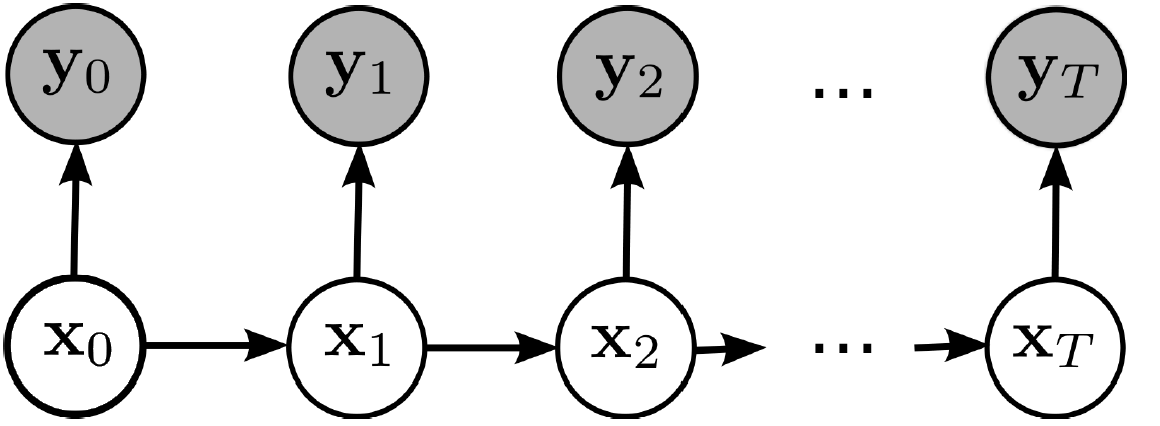
\includegraphics[width=0.7\textwidth]{hmm.png} 
\caption{Hidden Markov Models}
\label{fig:HMM}
\end{figure}

This class of models are designed to model evolving systems that output some observable events over time, which depends on the internal state of the system in a on-line manner. This imposes an implicit requirement on computation perspective: the estimate calculation cost should remain constant over time, i.e., the calculation cost does not increase with the increasing number of states.

Arguably, the most common inference problem in HMMs is the smoothing distribution, $p(x_{0:t} \mid y_{0:t})$, that is estimating the states $x_{0:t}$ based on the sequence of observations up to time $t$, $y_{0:t}$. Using Bayes rules, we can write the density of the distribution of interest in the recursion form as follows:
\begin{align}
    p(x_{0:t} \mid y_{0:t}) &= \dfrac{p(x_{0:t}, y_{0:t})}{p(y_{0:t})} \nonumber \\
                            &= \dfrac{p(x_{0:t-1}, y_{0:t-1})f(x_t \mid x_{t-1}) g(y_t \mid x_t)}{p(y_{0:t})} \nonumber \\ 
                            &= p(x_{0:t-1} \mid y_{0:t-1})\dfrac{f(x_t \mid x_{t-1}) g(y_t \mid x_t)}{p(y_t \mid y_{0:t-1})} 
\end{align}
This recursion is often re-written into two separate steps: the prediction step (the estimation of distribution of all states up to time $t$ given only states up to time $t-1$) and the update step (the correction of the predicted distribution taking into account the new observation) as follows:
\begin{align}
  p(x_{0:t} \mid y_{0:t-1}) &= p(x_{0:t-1} \mid y_{0:t-1})f(x_t \mid x_{t-1}) \nonumber \\
  p(x_{0:t} \mid y_{0:t})   &= \dfrac{p(x_{0:t} \mid y_{0:t-1}) g(y_t \mid x_t)}{p(y_t\
 \mid y_{0:t-1})}
\end{align}

Moreover, any smoothing distribution $p(x_{j:k} \mid y_{1:t})$ where $(0 \leq j \leq k\leq t)$ can be obtained by integrating out $x_i$ that are not interested in as follows:
\begin{equation}
  p(x_{j:k} \mid y_{0:t}) = \int p(x_{0:t} \mid y_{0:t}) dx_{0:j-1, k+1:t}
\label{eq:smoothing}
\end{equation}
A common smoothing distribution of interest is the marginal distribution at time $t$, $p(x_t \mid y_{0:t})$, which is also referred to as the filtering distribution.

Another distribution of interest is  the prediction distribution, that is the estimation of the distribution of any unseen \emph{future} states using only all observations up to current time. If we let $j = 0$ and $k \geq t$ in \eqref{eq:smoothing}, we obtain the following equation:
\begin{equation}
  p(x_{0:k} \mid y_{0:t}) = p(x_{0:t} \mid y_{0:t}) \prod^k_{i=t+1} f(x_i \mid x_{i-1})
\end{equation}
Therefore, any prediction density can be obtained by simply integrating out the variables of not interest from the above equation.

While these expressions \emph{appear} to be very simple, the distribution estimation problem is in fact far from being resolved in practice. The integrals involved in the above equations are often intractable and can only be estimated, since they require the evalution of complex high-dimensional integrals\footnote{Except under very special setting, in which the marginal filtering density $p(x_t \mid y_{0:t})$, the prediction density $p(x_n \mid y_{0:t-1})$ and the recursive likelihood $P(y_t \mid y_{0:t-1})$ are all Gaussian densities, then their means and variances can be computed analytically using Kalman Filter as shown in Appendix \ref{sec:KF}.}. 

\subsection{Sequential Important Sampling (SIS)}
\label{sec:SIS}
Sequential Monte Carlo provides a systematic way to approximate the solution to this estimation problem. Let assume that it is possible to decompose the selected proposal distribution into recursion form as follows:
\begin{align}
	q_{0:t}(x_{0:t} \mid y_{0:t}) &= q_{0:t-1}(x_{0:t-1} \mid y_{0:t-1}) q_t(x_t \mid x_{0:t-1}, y_{0:t}) \nonumber \\
	             &= q_0(x_0 \mid y_0) \prod^t_{i=1} q_i(x_i \mid x_{0:i-1}, y_{0:i})
\label{eq:q}
\end{align}
then it is possible to obtain sample ${x_{0:t}}$ by first sampling $x_0 \sim q_0(\cdot)$ at time $0$ and then $x_i \sim q_i(x_i \mid x_{0:i-1}, y_{0:i})$ for all time $i$ from $1$ to $t$. The corresponding weight associated to each sample $x_{0:t}$ can also be decomposed into recursion form as follows:
\begin{align}
  \tilde{w_t} &= \dfrac{p_{0:t}(x_{0:t} \mid y_{0:t})}{q_{0:t}(x_{0:t} \mid y_{0:t})} \nonumber \\
%              &= \dfrac{p_{0:t-1}(x_{0:t-1} \mid y_{0:t-1})}{q_{0:t-1}(x_{0:t-1} \mid y_{0:t-1})} \dfrac{p_{0:t}(x_{0:t} \mid y_{0:t})}{p_{0:t-1}(x_{0:t-1} \mid y_{0:t-1})q_t(x_t \mid x_{0:t-1}, y_{0:t})} \nonumber \\
%              &= \tilde{w}_{t-1} \dfrac{p_{0:t}(x_{0:t} \mid y_{0:t})}{p_{0:t-1}(x_{0:t-1} \mid y_{0:t-1})q_t(x_t \mid x_{0:t-1}, y_{0:t})} \nonumber \\
              &\propto \tilde{w}_{t-1} \dfrac{f_t(x_t \mid x_{t-1})g_t(y_y \mid x_t)}{q_t(x_t \mid x_{0:t-1}, y_{0:t})} \label{eq:w} \\
              &\propto \tilde{w}_0 \prod^t_{i=1} \alpha_i(x_{i})          
%  &= w_0(x_0) \prod^t_{i=1} \frac{p_i(x_{0:i})}{p_{i-1}(x_{0:i-1})q_t(x_i \mid x_{0:i-1})} \nonumber \\
\end{align}
where $\alpha_t(x_{t})$  is often referred to as incremental importance weight function. This is the key concept in SIS.

Using these weighted samples $\{(x^{(i)}_{0:t}, \tilde{w}^{(i)}_t)\}_{1 \leq i \leq N}$, it is possible to estimate any function $f$ defined on the space using the self normalised importance sampling estimator in the same way as \eqref{eq:is} as follows:
\begin{align}
  \hat{f}(x_{0:t}) &= \sum^N_{i=1} \dfrac{\tilde{w}^{(i)}_t}{\sum^N_{j=1}\tilde{w}^{(j)}_t} f(x^{(i)}_{0:t}) \nonumber \\
   &= \sum^N_{i=1} \hat{w}^{(i)} f(x^{(i)}_{0:t})
\end{align}
The SIS algorithm is summarised in Algorithm \ref{algo:sis}.

\begin{algorithm}
\caption{Sequential Importance Sampling}\label{algo:sis}
\begin{algorithmic}[1]
\Function{SequentialImportanceSampling}{N, T}
\State Set $t \gets 0$.
\State For $i \in 1, \ldots, N$, sample $x^{(i)}_0 \sim q(x^{(i)}_0 \mid y^{(i)}_0)$.
\State For $i \in 1, \ldots, N$, calculate the unnormalized importance weights:
\begin{equation*}
 \tilde{w}^{(i)}_0 = \dfrac{f(x_0^{(i)})g_0(y_0 \mid x^{(i)}_0)}{q_0(x^{(i)}_0)}
\end{equation*}
\State For $i \in 1, \ldots, N$, normalize the importance weights:
\begin{equation*}
\hat{w}^{(i)}_0 = \dfrac{\tilde{w}^{(i)}_0}{\sum^N_{i=1} \tilde{w}^{(i)}_0}
\end{equation*}
\State Set $t \gets t + 1$.
\While{$t \leq T$}
\State For $i \in 1, \ldots, N$, sample $x^{(i)}_t \sim q(x^{(i)}_t \mid y_{t-1}, x^{(i)}_{t-1})$.
\State For $i \in 1, \ldots, N$, set $x^{(i)}_{0:t} \gets (x^{(i)}_{0:t-1}, x^{(i)}_t)$.
\State For $i \in 1, \ldots, N$, calculate the unnormalized importance weights:
\begin{equation*}
 \tilde{w}^{(i)}_t = w^{(i)}_{t-1} \dfrac{f_t(x^{(i)}_t \mid x^{(i)}_{t-1})g_t(y_t \mid x^{(i)}_t)}{q_t(x^{(i)}_t \mid x^{(i)}_{t-1}, y_t)}
\end{equation*}
\State For $i \in 1, \ldots, N$, normalize the importance weights:
\begin{equation*}
\hat{w}^{(i)}_t = \dfrac{\tilde{w}^{(i)}_t}{\sum^N_{i=1} \tilde{w}^{(i)}_t}
\end{equation*}
\EndWhile
\EndFunction
\end{algorithmic}
\end{algorithm}

\subsection{Optimal Proposal Distribution}
While SIS is attractive, it is nothing but a specialised version of importance sampling introduced earlier in Section \ref{sec:IS}. As the state space increases with the number of time step $t$, direct importance sampling on a state space that is increasing in size is not very efficient. The weights of the samples will degenerate over time, in the sense that the weights start to concentrate only on a small number of samples. Consequently, many samples will have negligible weights and do not contribute much in the estimating the expectation. See \cite{JAM10} for a step-by-step illustration. The weight degeneracy issue cause the quality of the estimate degrades over time.

To alleviate this issue, looking at \eqref{eq:w}, it is obvious that the variance of importance weights can be minimised by using a proposal distribution of the following form:
\begin{equation}
 q_{t}(x_{t} \mid x_{t-1}, y_t) \propto f_{t}(x_{t} \mid x_{t-1}) g_{t}(y_{t} \mid x_t)
\end{equation}
This is often referred to as the optimal proposal distribution.

In general, it is not always possible to sample from this optimal proposal distribution. Yet, the knowledge of its form can be helpful in designing a reasonable good proposal distribution, which one can sample from. Better
proposal \emph{reduces} the amount of variance introduced, but it \emph{does not eliminate} the weight degeneracy problem.

\subsection{Sequential Importance Resampling (SIR)}
The variance in importance weights accumulates over iterations. This suggests a possible solution is to ``reset'' the weights associated to the samples somehow during the iterations \cite{JAM10}. Sequential Importance Resampling (SIR) introduces an additional resampling step to SIS step in a similar fashion as discussed in Section \ref{sec:IS}. After resampling, the weight of each sample is reset to be equal, i.e., $\frac{1}{N}$. This resampling step however introduces extra variance to the estimators.

A simple direct implementation of resampling step is to select the sample from the intermediate stage according to a Multinomial distribution with the success probability parameter set to the vector of normalised weights, $\hat{w}(x^{(i)})$, i.e., the chance of a sample point being replicated is proportional to its weight. 

There are many other resampling schemes have been proposed in the literature. For example, stratified resampling \cite{KG96} as the name suggested splitting the samples into strata to ensure the good coverage on the resulting sample set, residual resampling \cite{JSL98} which is able to decrease the variance of the weights due to resampling, etc. See \cite{DR05} for further details on the comparison of these sampling schemes.  The SIR algorithm is now summarised in Algorithm \ref{algo:sir}.

\subsection{Effective sample size (ESS)}
Resampling step induces additional Monte Carlo variance to the weights. Yet, this step is necessary to avoid accumulation of estimation variance onto the weights over time and therefore result in a more estimate.

To trade-off these two competing requirements, one possible way is to monitor the effective sample size (ESS) which provides a measure on the quality of the weighted samples. The ESS value can be estimated as follows:
\begin{equation}
  ESS \approx \dfrac{1}{E[w^2]} \approx \dfrac{\left(\sum^N_{i=0} w_i \right)^2}{\sum^N_{i=0}w_i^2}
\end{equation}

A common way to integrate this idea is to trigger the resampling step only if the $ESS_t$ fall below certain threshold at time $t$, say $\frac{N}{2}$. See \cite{JAM10} for further details on ESS.

\begin{algorithm}
\caption{Sequential Importance Resampling}\label{algo:sir}
\begin{algorithmic}[1]
\Function{SequentialImportanceResampling}{N, T}
\State Use Steps $2$-$11$ of Algorithm \ref{algo:sis}
\State \textbf{Resample:} For $i \in 1, \ldots, N$, resample $ x^{(i)}_{0:t} \sim \dfrac{\sum^N_{i=1}\hat{w}^{(i)}_t\delta_{x^{(i)}_{0:t}}}{\sum^N_{j=1} \hat{w}^{(j)}_t}$
\EndFunction
\end{algorithmic}
\end{algorithm}

\subsection{Resample-Move Algorithm}
\label{sec:rm}
However, resampling is not a silver bullet for sampling impoverishment. Essentially, resampling provides a mechanism to eliminate low weight samples to give way to replicate \emph{copies} of high weight samples. This allows all samples to participate and contribute to the distribution estimation. This is obvious beneficial for the case of estimating filtering distribution and predictive distribution. Over time, this replication result in decrease in the number of distinct samples for previous time steps. Eventually, many samples will have the share the same sample trajectory. This is a fundamental weakness of SMC, in which the sample path history is never re-written. This lose of diversity in the sample set will have a negative impact when it comes to any smoothing distribution estimation. 

To counteract this sample impoverishment, Resample-Move Algorithm \cite{BC01, WG01} is proposed to introduce some perturbation to the samples (so to diversify them) without changing the distribution they represent. This is accomplished by using MCMC steps with a Markov Kernel, $K$ that is invariant to the target distribution, $p(\cdot)$. In the original paper, this is achieved by simply introducing an additional MCMC ``move'' step to each sample after the resampling step using a kernel $K$  that is invariant to the target distribution. This Resample-Move algorithm is summarised in Algorithm \ref{algo:rm}.

This does not entirely solve the smoothing distribution estimation problem. To apply Markov Kernels with invariant distribution corresponding to the smoothing distribution, the space that Markov kernel is defined has to increase at each iteration. This implies the computation time increases linearly with time. Moreover, fast mixing high dimension Markov kernel in itself is not easy to design \cite{JAM10}.

To trade-off between the two requirements, one could adopt a sliding windows approach, in which MCMC Kernels which diversify the samples of the previous $n$ time step at each iteration. Adding this sliding window approach into the standard SIR algorithm will make each iteration has an additional \emph{fixed} computational cost.

\begin{algorithm}
\caption{Resample-Move Algorithm}\label{algo:rm}
\begin{algorithmic}[1]
\Function{ResampleMoveAlgorithm}{N, T}
\State Use Steps $2$-$11$ of Algorithm \ref{algo:sis}
\State \textbf{Resample:} For $i \in 1, \ldots, N$, resample $ x^{(i)}_{0:t} \sim \dfrac{\sum^N_{i=1}\hat{w}^{(i)}_t\delta_{x^{(i)}_{0:t}}}{\sum^N_{j=1} \hat{w}^{(j)}_t}$
\State \textbf{Move:} For $i \in 1, \ldots, N$, sample $x^{(i)}_{0:t} \sim K_t(\cdot)$, where $K_t$ is $p_t$-invariant.
\EndFunction
\end{algorithmic}
\end{algorithm}

\subsection{Rao-Blackwellised SMC}
\label{sec:msmc}
In practice, many models may not be entirely non-linear or non-Gaussian. Some states may be linear and Gaussian, conditional upon other states. Instead of naively modelling all state spaces using SMC, a better approach would be carrying out analytical computation as possible on the linear Gaussian states and use SMC model only the non-linear states. This marginalisation setting will yield estimate that has smaller variance.

To illustrate this, let consider the a simple conditional linear Gaussian Model as follows:
\begin{align}
  X^L_t &= A_t(X^N_t)X_{t-1} + B_t(X^N_t)W_t + F_t(X^N_t) \\
  Y_t &= C_t(X^N_t)X_t + D_t(X^N_t)V_t + G_t(X^N_t)
\end{align}
where $\{X^N_t\}_{t \geq 0}$ is a non-linear Markov processs, $A_t$, $B_t$, $C_t$, $D_t$, $F_t$, $G_t$ are appropriate matrix/vector of $X^N_t$ and  $\{W_t\}_{t \geq 0}$ and  $\{V_t\}_{t \geq 0}$ are independent sequences of standard Gaussian random variable, i.e., $W_t, V_t \sim \mathcal{N}(0,I)$. In such a case, the transition density and likelihood of this model are Gaussian distributions with center lied at a point of a linear combination of the known $x^N_t$ that can be obtained by using classical Kalman Fitering recursions as shown in Appendix \ref{sec:KF}.


The discussion here has been focused on conditional linear Gaussian model. The discrete state space HMMs is another important class of HMMs in which HMM forward algorithm \cite{LRR89} can be used to marginalise the internal states. See \cite{CO05} for further details.


\section{Conclusion}
This chapter presents a review of Monte Carlo methods, with a particular focus on Sequential Monte Carlo (SMC) used extensively in this thesis for portfolio optimisation. This chapter begins with a brief introduction on the traditional Monte Carlo sampling techniques. Then, it details the SMC, along with various extensions proposed to improve the performance of the algorithm.

It is worth to have a remark here that the SMC techniques are not only applicable to sequential filtering problem. For example, it has been established that it is possible to use SMC techniques within MCMC framework (pMCMC, where p stands for particle) \cite{CA10} to build high dimensional proposal distribution to improve standard MCMC. In the next chapter, we will show how SMC can be used as a maximiser to search for a optimal strategy for the optimal portfolio, given a multiplicative reward function.

% ------------------------------------------------------------------------


%%% Local Variables: 
%%% mode: latex
%%% TeX-master: "../thesis"
%%% End: 
